
\documentclass[11pt,a4paper]{report}
\usepackage{amsmath}
\usepackage{amsfonts}
\usepackage{amssymb}
\usepackage{graphicx}
\usepackage[left=2cm,right=2cm,top=2cm,bottom=2cm]{geometry}
\usepackage{listings}

\usepackage{xcolor}

\lstset{
    language=lisp,
    basicstyle=\ttfamily\small,
    aboveskip={1.0\baselineskip},
    belowskip={1.0\baselineskip},
    columns=fixed,
    extendedchars=true,
    breaklines=true,
    tabsize=4,
    prebreak=\raisebox{0ex}[0ex][0ex]{\ensuremath{\hookleftarrow}},
    frame=lines,
    showtabs=false,
    showspaces=false,
    showstringspaces=false,
    keywordstyle=\color[rgb]{0.627,0.126,0.941},
    commentstyle=\color[rgb]{0.133,0.545,0.133},
    stringstyle=\color[rgb]{01,0,0},
    numbers=left,
    numberstyle=\small,
    stepnumber=1,
    numbersep=10pt,
    captionpos=t,
    escapeinside={\%*}{*)}
}
\author{Fermin A. Ahumada Garcia}
\title{Reporte Tarea 2}
\begin{document}
\maketitle
\section*{Problema 5 }
\textbf{La llamada (bundle ’(”a” ”b” ”c”) 0) es un buen uso de bundle? ¿qué produce? ¿por qué?}\\
Este ejemplo en particular iba generar un bucle infinito, por que al llamar a \textit{drop} y \textit{take}, al ser  $n = 0$,hace que no recorra los elementos de esta,y nunca se vaciará.
\section*{Problema 9}
\textbf{Dibuja un diagrama como el de la figura anterior pero para la lista ’(11 9 2 18 12
14 4 1).}\\
\begin{figure}[ht]
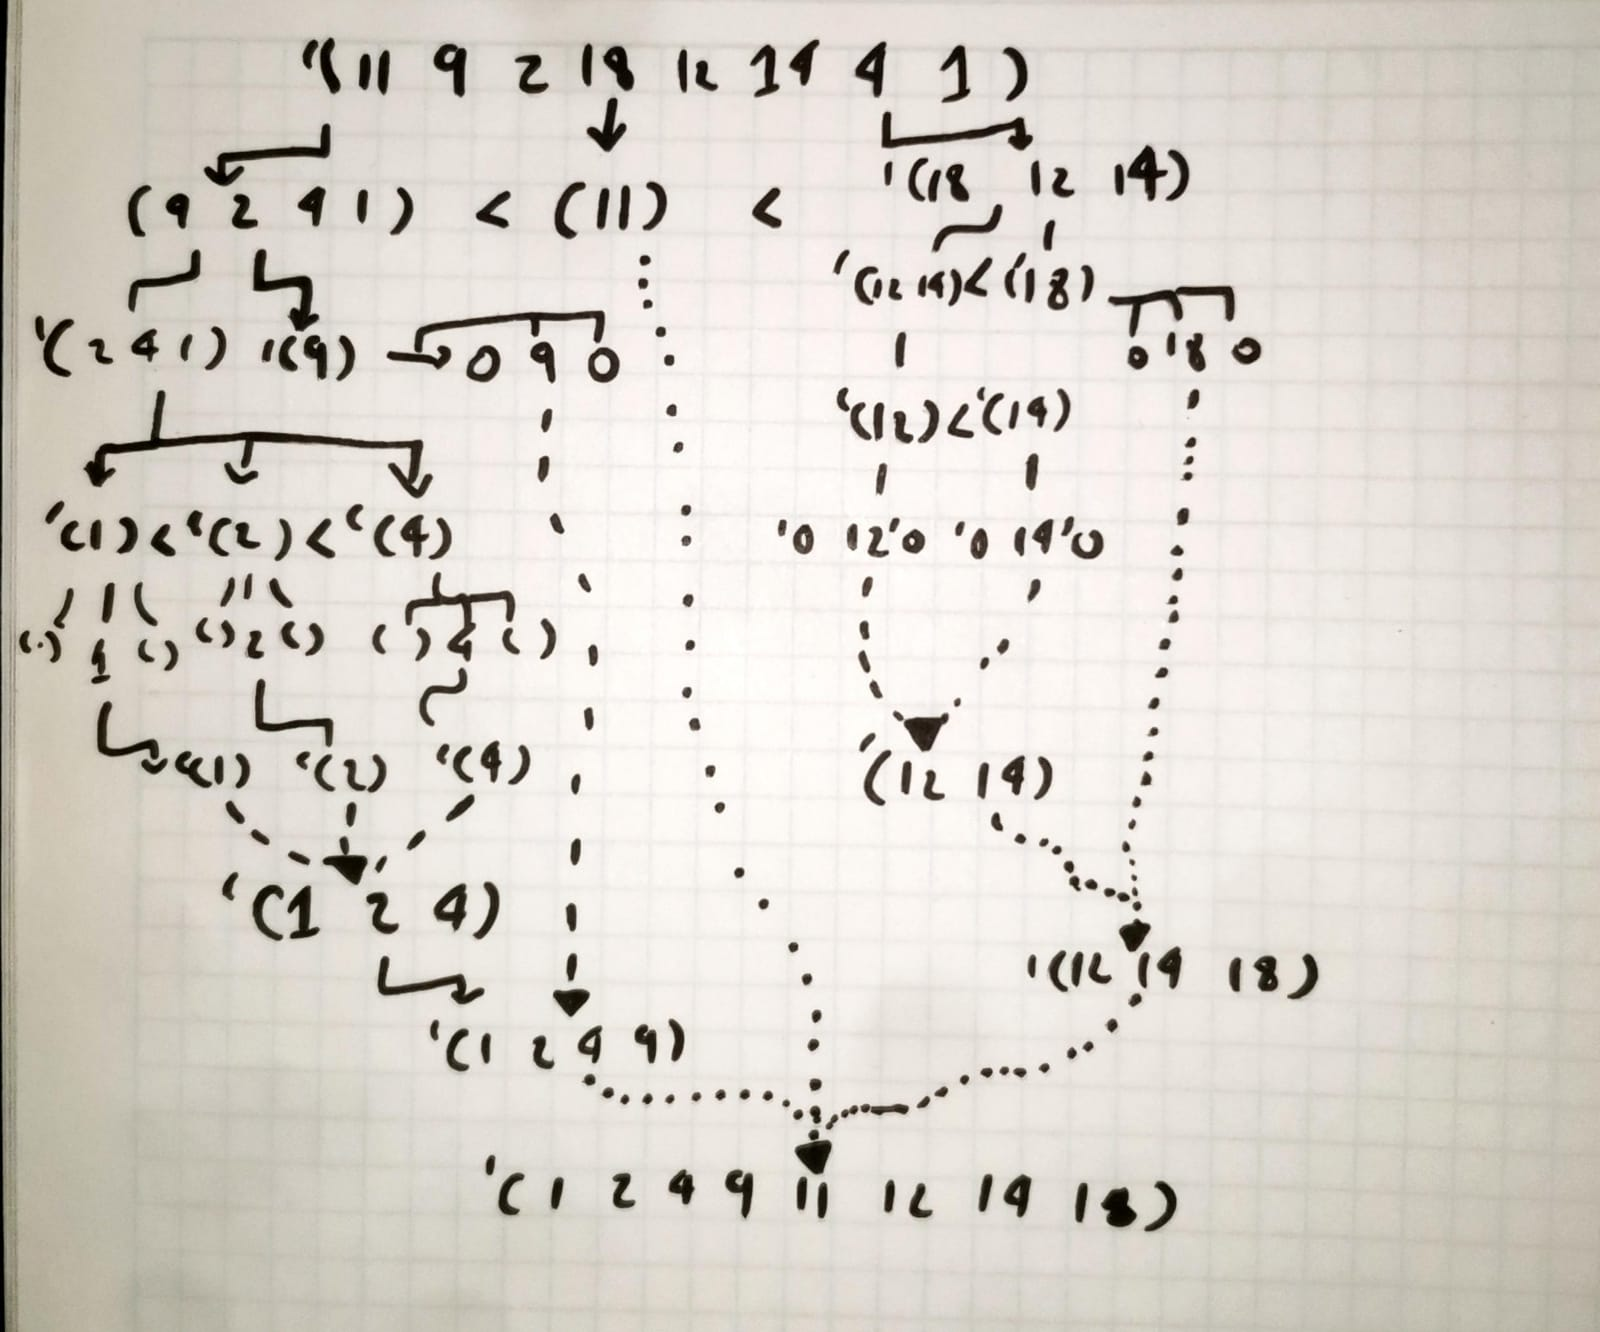
\includegraphics[width=15cm]{image}
\centering
\end{figure}
\section*{Problema 11}
\textbf{Si la entrada a quicksort contiene varias repeticiones de un número, va a regresar una lista estrictamente más corta que la entrada. Responde el por qué y arregla el problema.}\\
La entrada a quicksort al tener una gran cantidad de números repetidos,esta va a regresar una lista más corta que la entrada.
Al entrar en los métodos de \textit{largers} y \textit{smallers} solo agregan los elementos que cumplan al ser mayor o menor que el pivote.En algun punto de la recursión ,el pivote repetido estará en la lista ,lo cual el algoritmo lo va a ignorar por no saber que hacer con el.\\
Por eso se creo una función llamada \textit{eq},que ingresa estos valores repetidos .
\\\\\\\
\begin{lstlisting}
(define (eq ls n)
  (if (null? ls)
      null
      (cond
          [(eq? (first ls) n) (cons n (eq (rest ls) n))]
          [else (eq (rest ls) n)])))
\end{lstlisting}
Esta función filtrará a los resultados que son iguales de ls al pivot, y los agregará a una lista nueva, modificando \textit{quicksort} para juntar 3 listas

\end{document}